	%Template by Mark Jervelund - D1 - 2015 - mjerv15@student.sdu.dk

\documentclass[a4paper,10pt,titlepage]{report}

\usepackage[utf8]{inputenc}
\usepackage[T1]{fontenc}
\usepackage[english]{babel}
\usepackage{amssymb}
\usepackage{amsmath}
\usepackage{amsthm}
\usepackage{graphicx}
\usepackage{fancyhdr}
\usepackage{lastpage}
\usepackage{listings}
\usepackage{algorithm}
\usepackage{algpseudocode}
\usepackage[document]{ragged2e}
\usepackage[margin=1in]{geometry}
\usepackage{color}
\usepackage{datenumber}
\usepackage{venndiagram}
\usepackage{chngcntr}
\setdatetoday
\addtocounter{datenumber}{0} %date for dilierry standard is today
\setdatebynumber{\thedatenumber}
\date{}
\setcounter{secnumdepth}{0}
\pagestyle{fancy}
\fancyhf{}

\newcommand{\Z}{\mathbb{Z}}
\lhead{Database Management Systems (DM556))}
\rhead{Mark Jervelund (Mjerv15) Troels B. Petersen (trpet15)}
\rfoot{Page  \thepage \, of \pageref{LastPage}}
\counterwithin*{equation}{section}

\lstset{
  numbers=left,
  stepnumber=5,
  firstnumber=1,
  numberfirstline=true
  frame=single,
  breaklines=true,
  postbreak=\raisebox{0ex}[0ex][0ex]{\ensuremath{\color{red}\hookrightarrow\space}}
}

\begin{document}
\begin{titlepage}
\centering
    \vspace*{9\baselineskip}
    \huge
    \bfseries
    Project 3\\

    \normalfont
	\huge
    Database Management Systems (DM556)  \\[4\baselineskip]
    \normalfont
	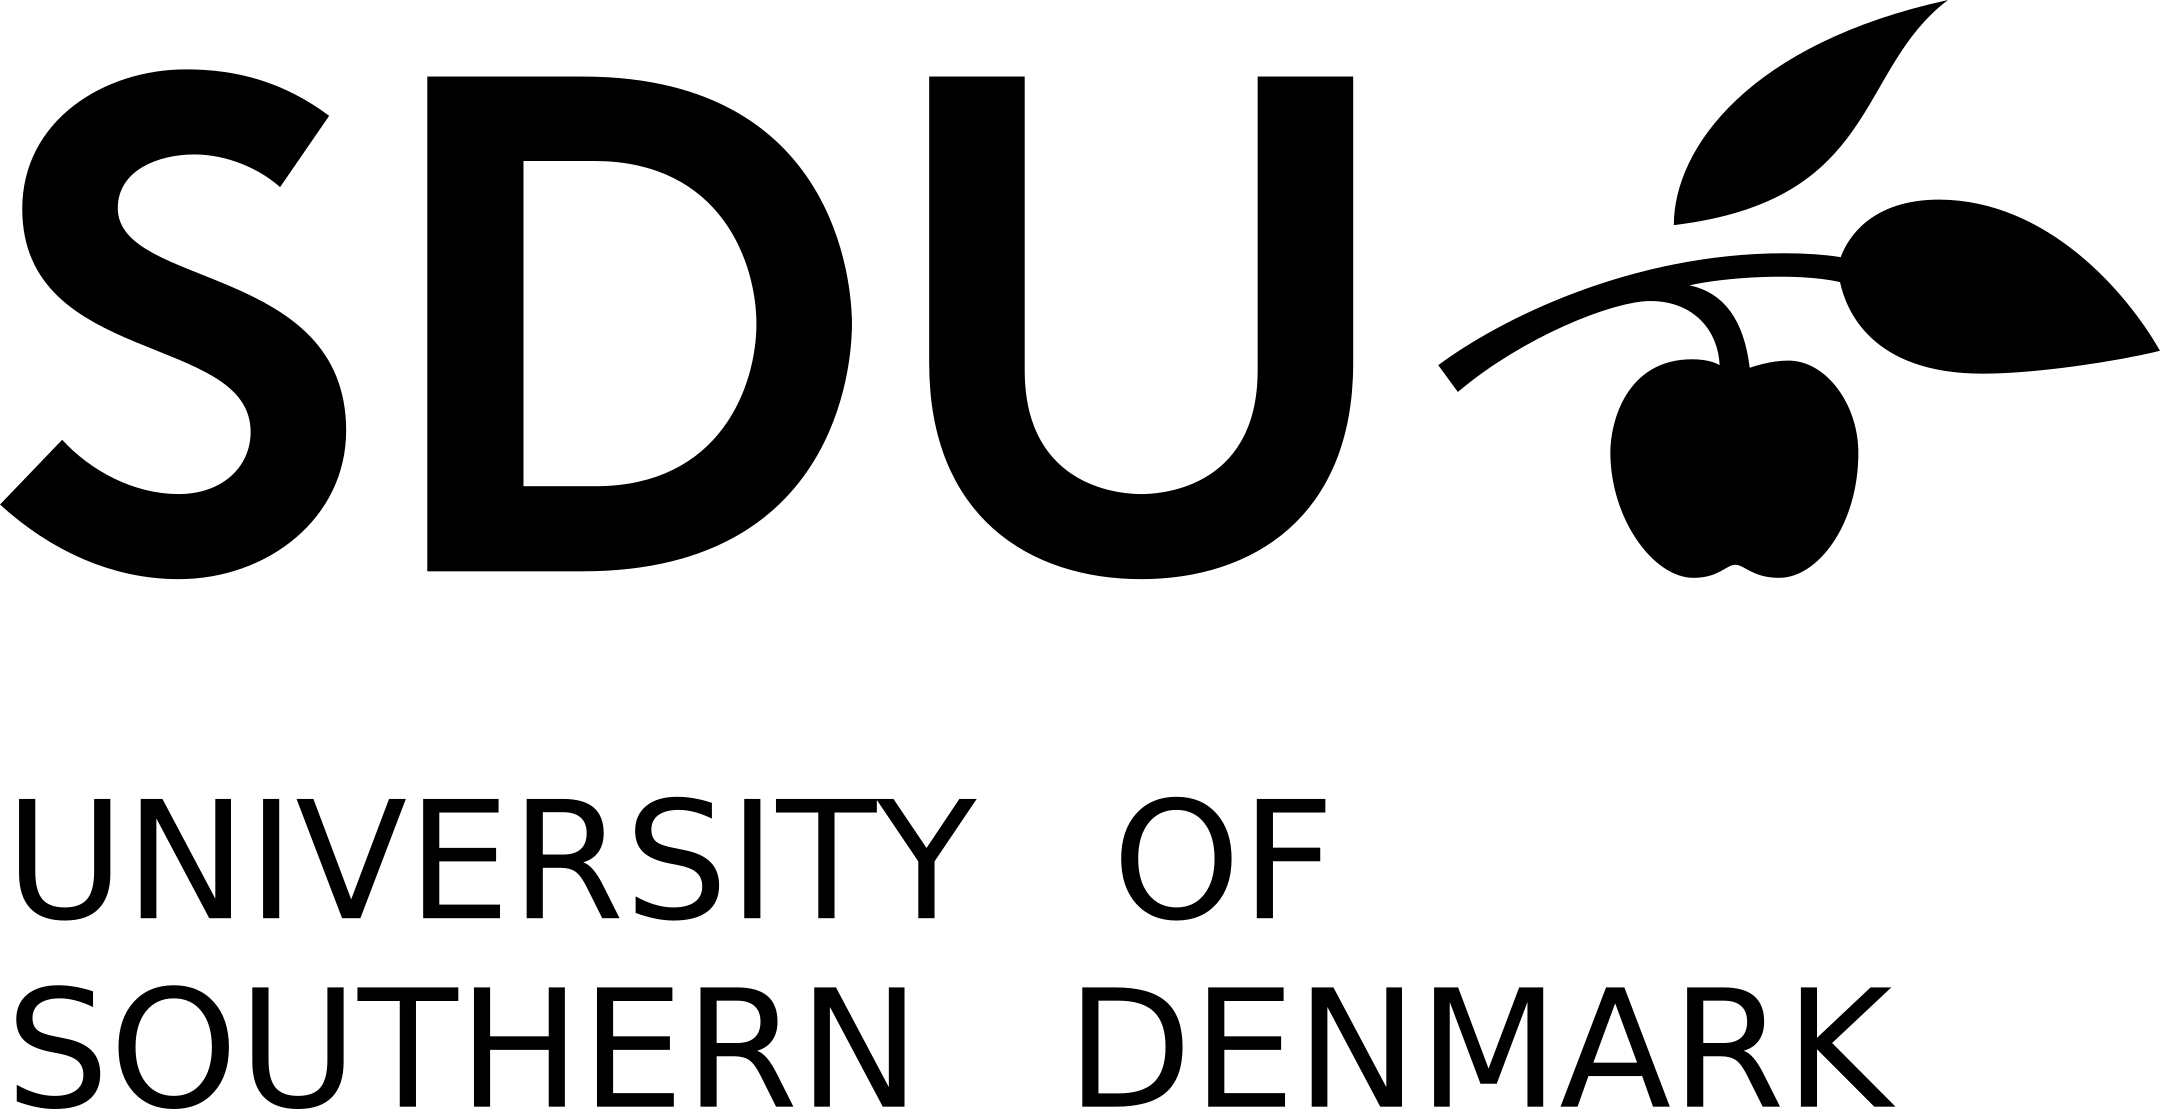
\includegraphics[scale=1.5]{SDU_Logo}
    \vfill\
    Group 2\\
    Mark Jervelund (Mjerv15)    Troels B. Petersen (trpet15)
    \vspace{5mm}
    IMADA \\
    \textbf{\datedate} \\[2\baselineskip]
\end{titlepage}
%\renewcommand{\thepage}{\roman{page}}% Roman numerals for page counter
%\tableofcontents

%\newpage
\setcounter{page}{1}
\renewcommand{\thepage}{\arabic{page}}

\lstset{language=Java}          % Set your language (you can change the language for each code-block optionally)

\section{Project 1}
BuffMgr.java and clock.java in bufmgr \\


\subsection{bufMgr.java} 

\subsubsection{public bufmgr(int numbufs)}
init function that initializes the bufpool and the frame tap. as well as building the pagemap and selecting the replacement function.
\subsubsection{public PageId newPage(Page firstpg, int run\_size)}
Loads a new page into the buffer pool, and calls the pinpage function on the first page, if sucssesful calls the replacer to put the page in the frametab, and returns the pageid id. or throws RuntimeException if it fails to pin the page.

\subsubsection{public void pinPage(PageId pageno, Page page, boolean skipRead)}
Pins a disk page into the buffer pool. If the page is already pinned,
this simply increments the pin count. Otherwise, this selects another
page in the pool to replace, flushing the replaced page to disk if
it is dirty.
\vspace{5mm}
\\
If one needs to copy the page from the memory instead of reading from
the disk, one should set skipRead to PIN\_MEMCPY. In this case, the page
shouldn't be in the buffer pool. \\ Throw an IllegalArgumentException if so. )

\subsubsection{  public void unpinPage(PageId pageno, boolean dirty) throws IllegalArgumentException }
Unpins a disk page from the buffer pool, decreasing its pin count. and marks it as dirty in the pagemap if the boolean dirty is true.
\vspace{5mm}

\subsubsection{public void flushPage(PageId pageno}
Flushes a single page to disk if dirty, else just does nothing.

\subsubsection{public void flushAllPages(}
Calls the flush page on all pages in the buffer to disk using the flush page function so only the dirty ones get written.

\subsubsection{public void getNumBuffers}
return the length of the buffer pool

\subsubsection{public int getNumUnpinned}

Loops over the frame tab and counts how many pages are pinned at any given time.

\vspace{5mm}
\subsection{clock.java} 
pickvictim \\
Gets the first page in the frametab with pincount 0. \\
This means that we remove the first page in the buffer that no one else is using, if there are no free pages then we return -1 and signalling the parent function that there is no free pages in the buffer pool at the moment.

\newpage
\section{Project 2}

\subsection{projection.java} 
\subsubsection{ public Projection(Iterator iter, Integer... fields) }
Makes a new table where the columns we want to select. \\
	GetNext gets the next via the iterator and only selects the fields in tuple.

\subsection{selection.java}

The selection works mostly the same way as out projection. the main difference is that when we check for HasNext we compare with the predicate, if there is a valid tuple, we store this in a variable until get next is called.
\\
our getNext then returns the tuple stored by hasnext and sets the variable its stored in to null.


\subsection{Sort.java}

 
\subsection{Mergejoin.java}
 
Merge join assumes that both inputs are sorted.
It works by using hasNext. It iterates though the "left" input and compares it with the right input. Every time the left input matches the right input, it joins these two.

\newpage
\section{Project 3}
\subsection{select.java}
\subsubsection{Parser}
checks if the query is valid, this is done by using the QueryCheck function built into the miniDBMS system.
\subsubsection{Optimizer1}
naive\\
Cross joins all tables first \\ then selects all valid tuples, and lastly we project the selected columns from the resulting table.

\subsubsection{Optimizer2}

we build the tree dept first, by looping over the tables to load, and at the same time we check if any of the predicates are valid on any of the individual tables.
This is done by using the Querycheck function to check if the matching predicates and tables are valid, if they are it's added to the iterator, and the predicate is removed from the predicate list. after this is done for all joins.
ZZ
We apply the remaining selections to the top of the tree, and then perform the projection.


\subsection{delete.java}

Delete selects all the records to be deleted based on the predicate. 

It does so by iterating through the selection and adding the selected records to the delete list. We add the record-ID to the delete list. This is so that we can remove the entry from the hashIndex.

However, it has not been removed from the database yet. This is done later, where we use the deleteIterator, that is based on the deletelist.

\subsection{update.java}

Very similar to delete, however update inserts a new entry in the hashindex after removing, then updating the information in the heapfile using the update record method in the heapfile data structure, after this is done the key is inserted back into the hashindex. 






\end{document}